\chapter{Quantum-dot cellular automata}

\graphicspath{{../gfx/chapter01/}}

\begin{figure}
  \center
  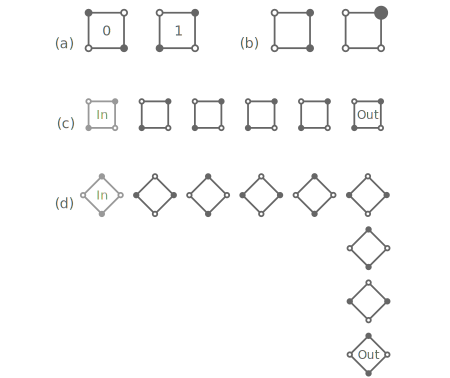
\includegraphics{intro_qca}
  \caption{\ldots}
  \label{fig:intro_qca}
\end{figure}

Lent et al.\ introduced the concept of quantum-dot cellular automata as an
alternative computing paradigm in 1993 \cite{lent1993quantum}. Thus the aim was
a novel physical scheme to build digital circuits that would overcome some of
the limitations of CMOS technology, promising potentially lower power
consumption, higher device density, and faster clocking. As the name alludes to,
quantum-dot cellular automata (QCA) is built from quantum-dots which are grouped
together in cells. Figure~\ref{fig:intro_qca}(a) shows a basic QCA cell. Four
quantum dots are arranged on the corners of a square. The dots are idealized as
perfectly localized single orbitals on a perfectly decoupled non-intrusive
medium. Therefore, each dot can be occupied by up to two electrons. In the QCA
scheme, however, each cell is occupied by only two electrons in total. The cell
is quarter-filled. The electrons tunnel between different dots in a cell, but
the dominant energy scale is set by the Coulomb repulsion between the particles.
Simply by virtue of the Coulomb repulsion, and ignoring the comparatively small
tunnelling for now, the diagonal states, Fig.~\ref{fig:intro_qca}(a), are the
two energetically preferred electron configurations. In comparison, edge states
or doubly occupied quantum dots are unfavourable higher energy states,
Fig.~\ref{fig:intro_qca}(b). A priori the two diagonal states are energetically
degenerate, but this degeneracy can be lifted by introducing an external Coulomb
potential, for example a second nearby QCA cell. Then these two states can be
identified with logic 0 and 1, as indicated in the figure.

A single cell by itself is, of course, not very interesting. Thus, multiple
cells can be positioned next to each other, for example as a straight line of
cells, Fig.\ref{fig:intro_qca}(c). The approach now again assumes that Coulomb
is the driving force and that electron tunnelling between cells is very small
and ideally zero. For a straight line of cells, these long-ranging, unscreened
Coulomb forces will tend to align the electron configurations of adjacent cells.
If the first cell is in logic state 1 then the second cell will also prefer
logic state 1 and so will in turn all the other cells in the line. The situation
is the same for logic state 0. Therefore, a straight line of cells is similar to
a wire not only in geometry, but also in functionality: It transmits a digital
signal. The same is true, with slight modifications, for a diagonal line of
cells --- cells rotated by $45^{\circ}$---, Fig.~\ref{fig:intro_qca}(d). In this
case the signal alternates from cell to cell, that is, logic 1 will follow logic
0 which followed from logic 0, and this again is simply by virtue of the
dominant Coulomb interactions between electrons on different cells. By using an
even number of cells the diagonal line of cells works as a wire just as well as
a straight line of cells. The pictogram also demonstrates a $90^{\circ}$ for the
diagonal line of cells which our newly gained intuition for these Coulomb-driven
systems expects to pose no problem for signal transmission.

The main idea of the QCA approach becomes apparent: Ideally bistable cells
interact with each other solely by Coulomb repulsion. By arranging the cells in
clever geometries we can realize interesting functionalities. One such clever
geometrical arrangement is the majority gate, Fig.~\ref{fig:intro_qca}(e). The
gate has three inputs which ``vote'' on the central cell. The majority wins and
sets the single output. The device is commonly operated with one fixed input,
for example $I_3 \doteq 0$ or $I_3 \doteq 1$. In the first case, $I_3 \doteq 0$,
the device functions as an AND gate for the remaining two inputs, $O = I_1 \land
I_2$. In the second case, $I_3 \doteq 1$, it is an OR gate with $O = I_1 \lor
I_2$. Now, the only missing piece for Boolean algebra is negation, $O = \lnot
I$. We had already seen that simply arranging cells at an $45^{\circ}$ angle as
in the diagonal line of cells above negates the signal from cell to cell. The
inverter, Fig.~\ref{fig:intro_qca}(f) recasts this idea into a more robust
layout. With that we have, at least in principle, all the necessary building
blocks for Boolean algebra and thus digital circuitry.

Conceptually, it is most elegant to set the inputs to a QCA circuit via driver
cells --- cells that resemble the QCA cell in form, but are made up from static
point charges instead of quantum dots. These static charges are thought to be
manipulatable to vary the input smoothly from the logic 0 to the logic 1 state.
In figure~\ref{fig:intro_qca} these driver cells are represented in light grey.
Of course, in practice such driver cells would be difficult if not impossible to
implement and the input would more likely be set by leads that provide the
necessary perturbative electrostatic field. The output of a QCA device can be
directly read from its output cells. In practical implementations this will
require a non-trivial charge probing apparatus.

Changing the input for a QCA device throws the system into an excited,
non-equilibrium state. The system will then dissipatively propagate to its new
ground state. For the given inputs, this ground state corresponds to the
solution of the computational problem the circuit is designed to solve. Let us
emphasize this: In QCA, the computational solution maps directly to the physical
ground state! At all times during performing a computation, the system is
relatively close to its ground state. Only a few charges move locally, in each
cell. QCA is a truly current-free approach and consequently inherently
low-power, especially when compared with CMOS technology. But the operation
close to the ground state also raises concerns for the operational temperature
for these devices. It is clear that for applications we would want to engineer
the system so that the energy gap between the ground state and the low-lying
excited states far exceeds room temperature.

It is difficult to derive general expectations for the clocking speed of QCA
circuits. The switching speed of a majority gate, for example, will greatly
depend on the system's parameters, but particularly on the nature of the
dissipative coupling of the circuit to its environment. A small dissipative
coupling will have the output polarization oscillating before it eventually
settles to its correct value. A very dissipative system in contrast might get
stuck in meta-stable states. Different material systems provide different
dissipative channels and modelling them quantitatively or even qualitatively
correctly is very challenging. We can make the circuit's operation less
dependent on the details of the dissipative processes and its dynamics more
controlled by introducing the concept of adiabatic switching, where parameters
are changed slowly enough for the system to always remain in its (instantaneous)
ground state. An applied gate voltage is used to raise or lower the tunnelling
barrier between the quantum dots, effectively freezing or delocalizing the
electrons. In principle, setting the device's inputs synchronously with the
varying gate voltage and fine-tuning the timing with respect to the QCA system's
intrinsic time-scales, allows a well-defined switching behaviour. In practice,
this is likely easier said then done and, additionally, for truly adiabatic
switching the switching times might be very long.

Even when the switching is not quite adiabatic introducing this effective
clocking scheme is very beneficial. We can partition large circuits into smaller
parts, which are clocked separately, thus pipelining computations from part to
part. This is important for building realistically large circuits. Even more
importantly, we really need to partition large systems into smaller pieces for a
more fundamental reason: As a simple example, we can consider a long wire and
introduce a defect, that is, we have two domains, one with logic 0 state and the
other with logic 1 state. This domain wall introduces an energy gap and this
will be the first excited state, whereas the one-domain completely ordered state
is the ground state. However, it is clear that the entropy of this first excited
state is increasingly larger for increasingly longer wires. Thus in the
thermodynamic limit the wire will be disordered even for infinitesimal
temperatures. Therefore, for a wire to reliably transmit a signal, we have a
maximum wire length, which depends on the operational temperature and the energy
gap to the first excited state. TODO





Let us note that QCA is a not a cellular automata in a strict mathematical sense,
but only by analogy to the idea of interacting cells.



quadrupole

TODO: How does the applied gate voltage control the tunnelling barrier?
Graph for the adiabatic switching / gates.
